
\ignore{One of the main problems, in many computer vision application, is to estimate a continuous real-valued function or a structured-output function from input features.} Estimation of a continuous real-valued or a structured-output function from input features is one of the critical problems that appears  in many machine learning  applications. Examples include predicting the joint angles of the human body from images, head pose, object viewpoint, illumination direction, and a person's age and gender. Typically, these problems are formulated by a regression model.  Recent advances in structure regression encouraged researchers to adopt it for formulating various problems with high-dimensional output spaces, such as segmentation, detection, and image reconstruction, as regression problems. However, \ignore{they are constrained by }the computational complexity of the state-of-the-art regression algorithms limits their applicability for big data\ignore{ that are used to compute the predictions}. In particular,  kernel-based regression algorithms such as Ridge Regression~\cite{ridgeReg70}, Gaussian Process Regression (GPR)~\cite{Rasmussen:2005}, and the Twin Gaussian Processes (TGP)~\cite{Bo:2010} require inversion of kernel matrices ($O(N^3)$, where $N$ is the number of the training points), which limits their applicability for big data. We refer to these non-scalable versions of GPR and TGP as full-GPR and full-TGP, respectively.
 
 %this should move elsewhere.
 %From data bias perspective, Yamada et al \cite{Yamada:2012}, proposed a co-variance shift adaptation algorithm and applied on Kernel regression (KR)~\cite{kernelReg03} and TGP, by incorporating importance weighting to the training points based on the training and test distributions. However, their approach gives the best prediction on TGP, which requires matrix inversion in both its weight and unweighted versions. .   



%Many machine learning tasks are constrained by computational time of the state-of-the-art algorithms, required to compute the prediction. For instance,  Gaussian Process Regression (GPR)~\cite{Rasmussen:2005}, Ridge Regression \cite{ridgeReg70}, Twin Gaussian Processes (TGP)~\cite{Bo:2010} which require inversion of Kernel matrices ($O(N^3)$, $N$ is the number of the training points ), which limits its applicability for large scale data. From data bias perspective, Yamada et al \cite{Yamada:2012}, proposed a co-variance shift adaptation algorithm and applied on Kernel regression (KR)~\cite{kernelReg03} and TGP, by incorporating importance weighting to the training points based on the training and test distributions. However, their approach gives the best prediction on TGP, which requires matrix inversion in both its weight and unweighted versions.

%\begin{figure}{r}{0.43\textwidth}
\begin{comment}
\begin{figure}
%\centering
%\begin{tabular}{cc}
%\bmvaHangBox{\fbox{
\includegraphics[width=0.21\textwidth]{nonOverlappingFig.png}
%\bmvaHangBox{\fbox{
\includegraphics[width=0.21\textwidth]{OverlappingFig.png}%\\
%(a)&(b)s
%\end{tabular}
\caption{24 points, Left: 3 disjoint kernel machines of 8  points,  Right: 5 Overlapping kernel machines of 8 points. $f_i(\mathbf{x}^*)$ is the $i^{th}$ kernel machine prediction for $\mathbf{x}^*$ test point.}
\label{fig:overlapandnonoverlap}
\end{figure}
\end{comment}




Khandekar et. al. \cite{khandekar2014advantage} discussed properties and  benefits of overlapping clusters for minimizing the conductance from spectral perspective. These properties of overlapping clusters also motivate studying scalable local prediction based on overlapping kernel machines.  Figure~\ref{fig:overlapandnonoverlap_ex} illustrates the notion by starting from a set of points, diving them into either disjoint and overlapping subsets, and finally learning a kernel prediction function on each (i.e., $f_i(x^*)$ for subset $i$, $x^*$ is testing point). \ignore{Our method is accurate and scalable as demonstrated in the experiments on 3-datasets (including Human3.6M, the largest human-3D-pose dataset).}
\textit{In summary, the main question, we  address in this paper, is how local kernel machines with overlapping training data could help speedup the computations and gain accurate predictions. We achieved considerable speedup and good performance on GPR, TGP, and IWTGP (Importance Weighted TGP) applied to 3D pose estimation datasets\ignore{; our framework firstly achieves quadratic prediction complexity for TGPs}. To the best of our knowledge, our framework is the first to achieve quadratic prediction complexity for TGP. The ODC concept is also novel in the context of kernel machines and is shown here to be successfully applicable to multiple kernel-machines\ignore{, resulting in a considerable speedup and an accurate prediction}}. We studies in this work GPR and TGP and IWTGP  (a third model) kernel machines\ignore{ (denoted by SM in the rest of the paper)}. The remainder of this paper is organized as follows: Section ~\ref{sec:2}  and~\ref{sec:relappmethod} presents some motivating kernel machines and the related work. Section ~\ref{sec:3} presents our approach and a theoretical justification for our ODC concept. Section ~\ref{sec:6} and \ref{sec:7} presents our experimental validation and conclusion.

\begin{comment}
There are five main contributions to this paper:
\begin{enumerate}[noitemsep,topsep=0pt,parsep=0pt,partopsep=0pt,leftmargin=*]
\item{Persistent prediction on boundaries is achieved our domain set cover notion.}
\item{As a first step of the (OD) cover computation, we propose a variant of K means algorithm to use for domain decomposition with equal number of points per cluster.}
\item{Our Overlapping Domain Cover notion is not restricted
to GPR. It is applicable various kernel machines (\eg TGP,
kernel regression).}
\item{$O(N^2)$ complexity is achieved for TGP and IWTGP local prediction under our framework.}
\item{We conducted experiments on three 3D-pose estimation datasets to validate our method.}
\end{enumerate}
\end{comment}
\begin{comment}
Section ~\ref{sec:2} present example kernel machines that benefits from our approach. Section ~\ref{sec:} presents an overview of our domain. Section ~\ref{} presents that training phases which involves  
\end{comment}
\begin{comment}
Performance advantages of our approach are detailed in the experiential results section. The remaining of this paper is organized as follows. Section 2 presents The domain decomposition framework, Section 3 and 4 detail the training and prediction phases. Section 5 presents the IWTGP integration under our framework. Section 6 presents experimental results. Finally, Section 7 presents the conclusion and future work.
\end{comment}
%\begin{figure}[t!]
%\centering
%    \begin{subfigure}[b]{0.19\textwidth}
%    \includegraphics[width=1.0\textwidth,height=0.75\textwidth]{nonOverlappingFig.png}
%    \vspace{-5mm}
%               \caption{$\,\,$}
%                \label{fig:nonoverlapping}
%        \end{subfigure}%
%        \begin{subfigure}[b]{0.19\textwidth}
%   \includegraphics[width=1.0\textwidth,height=0.75\textwidth]{OverlappingFig.png}
%       \vspace{-5mm}
%                \caption{$\,\,$}
%                 \label{fig:overlapping}
%        \end{subfigure}
%        \vspace{-4mm}
%        \caption{24 points (a) 3 disjoint kernel machines of 8  points, (b) 5 Overlapping kernel machines of 8 points. $f_i(\mathbf{x}^*)$ is the $i^{th}$ kernel machine prediction for $\mathbf{x}^*$ test point.}
%        \label{fig:overlapandnonoverlap}
%           \vspace{-6mm}
%\end{figure}


%\begin{figure}
%\centering
%\begin{tabular}{cc}
%\bmvaHangBox{\fbox{
%\includegraphics[width=2.8cm]{nonOverlappingFig.png}}}&
%\bmvaHangBox{\fbox{\includegraphics[width=2.8cm]{OverlappingFig.png}}}\\
%%\bmvaHangBox{\fbox{\includegraphics[width=5.6cm]{OverlappingFig.png}}}\\
%(a)&(b)
%\end{tabular}
%\caption{24 points (a) 3 disjoint kernel machines of 8  points, (b) 5 Overlapping kernel machines of 8 points. $f_i(\mathbf{x}^*)$ is the $i^{th}$ kernel machine prediction for $\mathbf{x}^*$ test point.}
%\label{fig:overlapandnonoverlap}
%\end{figure}

\begin{figure*}[t]
\centering
%\centering
%\begin{tabular}{cc}
%\bmvaHangBox{\fbox{
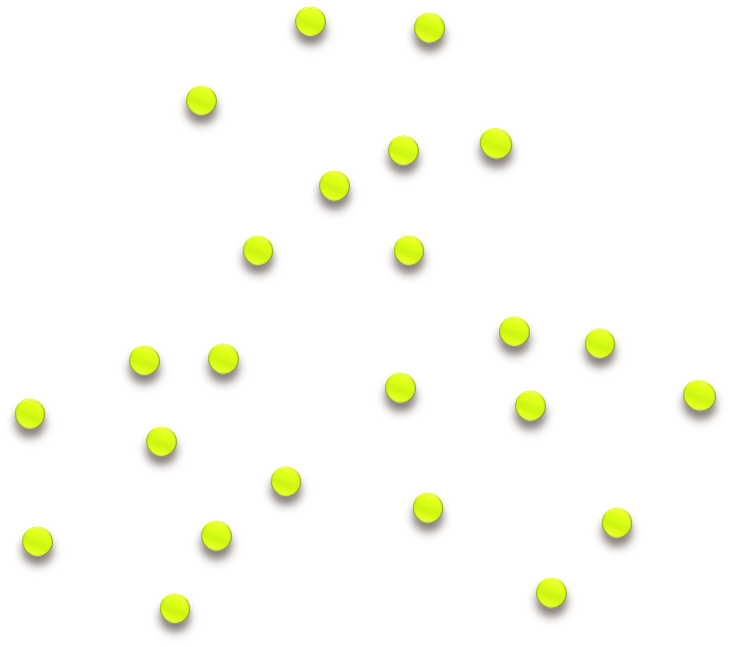
\includegraphics[width=0.31\textwidth]{ODC_intro_1.png}
%\bmvaHangBox{\fbox{
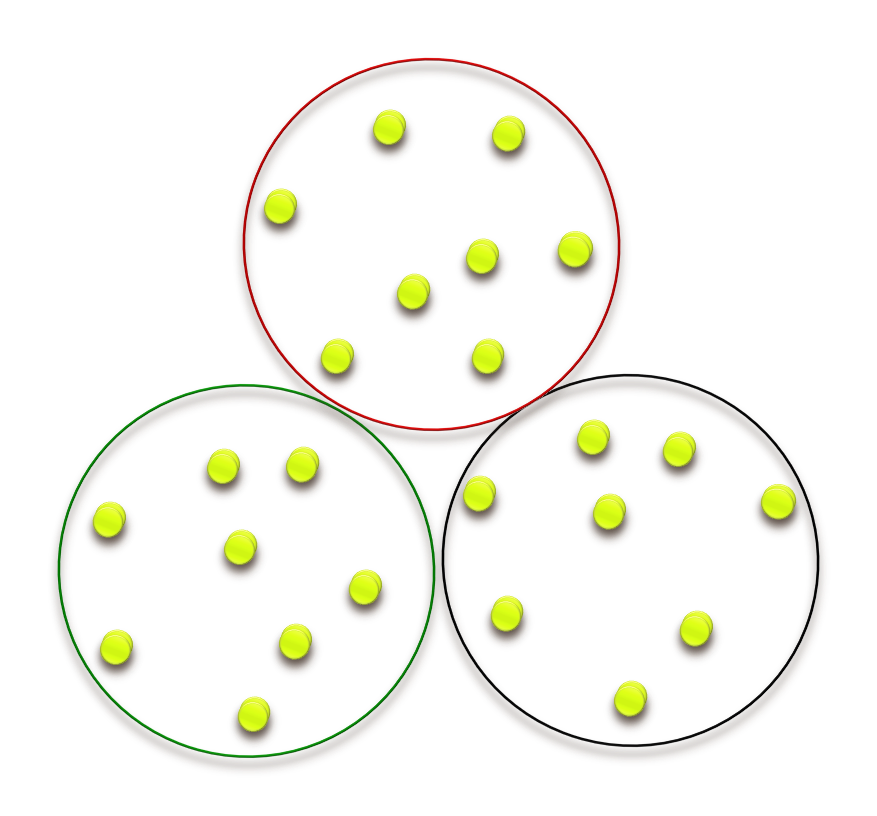
\includegraphics[width=0.31\textwidth]{ODC_intro_2.png}%\\
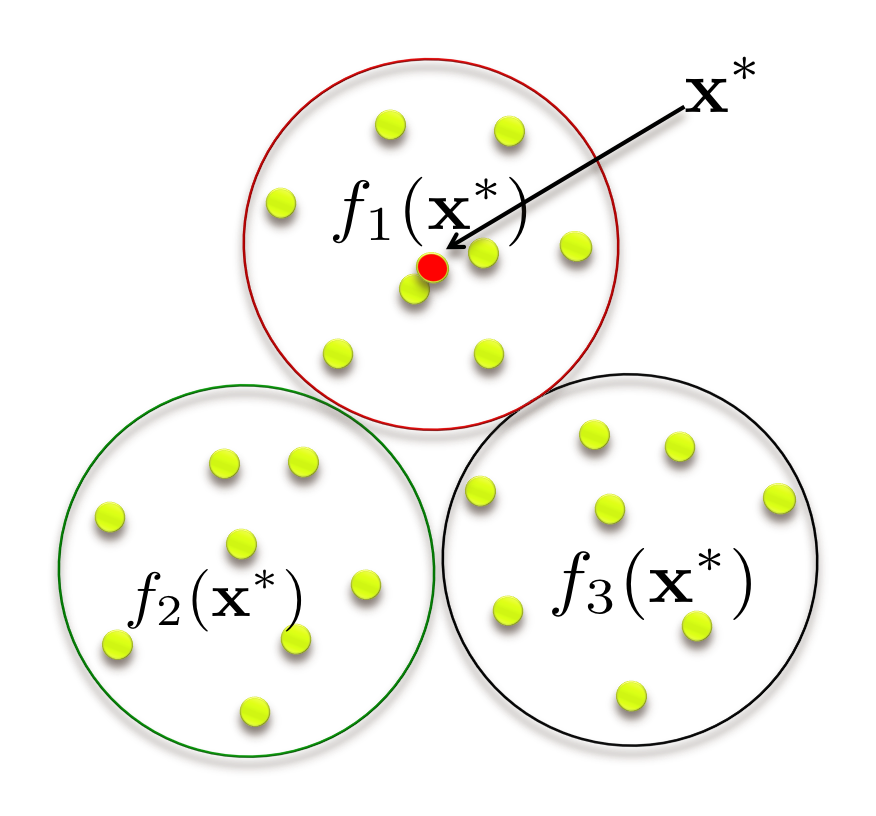
\includegraphics[width=0.31\textwidth]{ODC_intro_3.png}
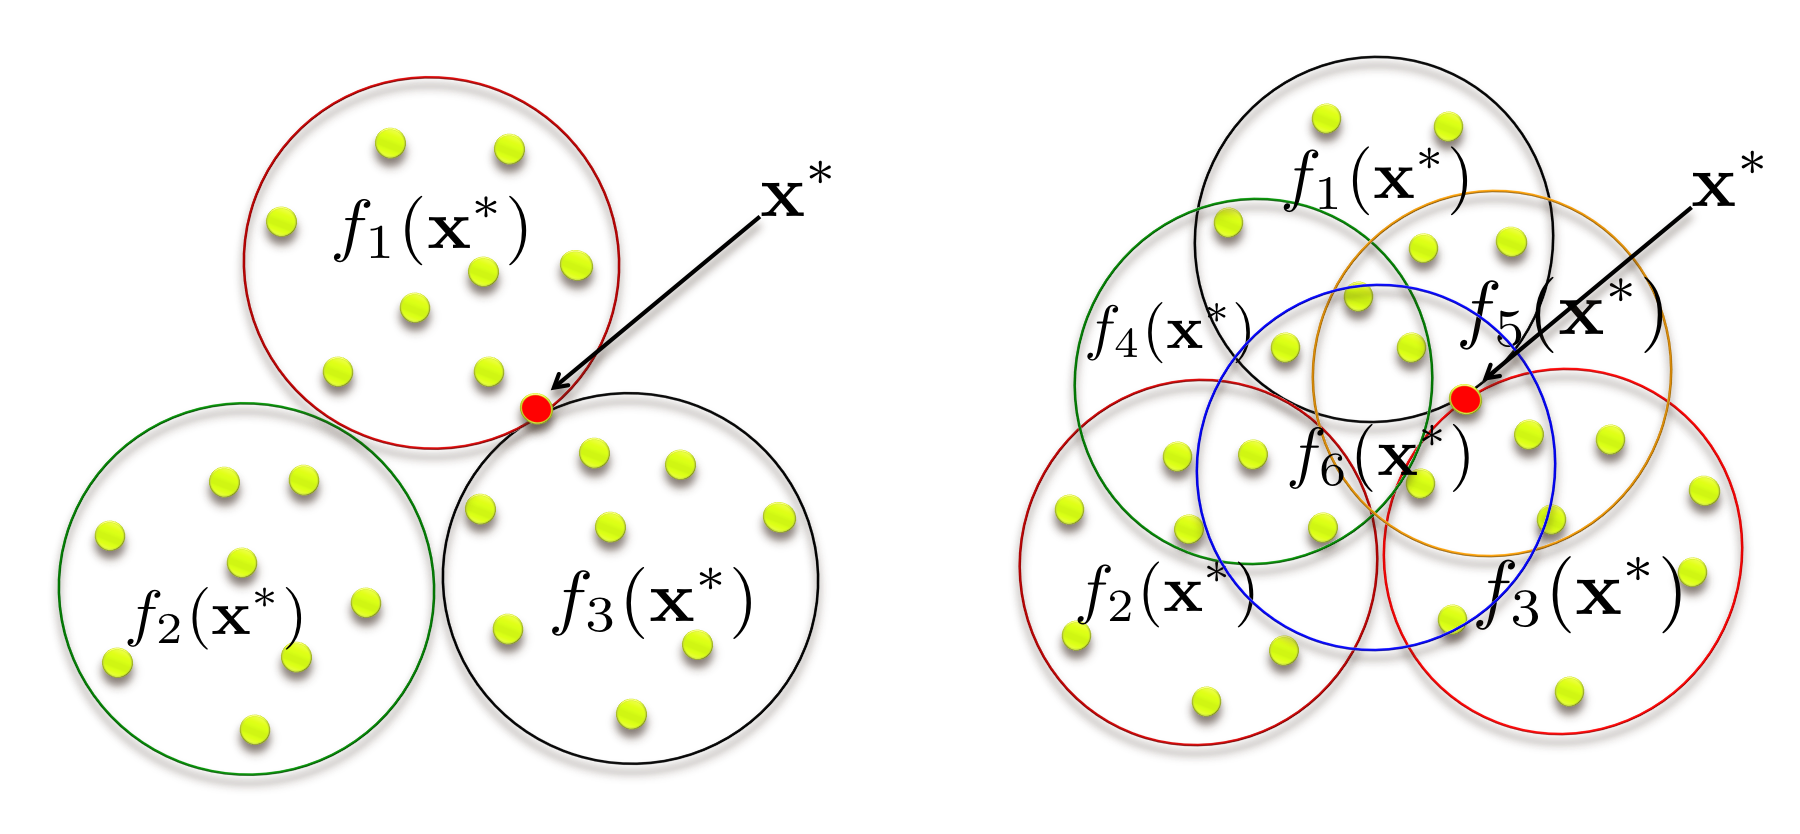
\includegraphics[width=0.62\textwidth]{ODC_intro_4.png}
%(a)&(b)s
%\end{tabular}
\caption{\textbf{Top}: Left:24 points, Middle: Overlapping Cover, Right: disjoint kernel machines of 8  points (evaluating $x^*$ near a middle of a kernel machine).  \textbf{Bottom}: Left: disjoint kernel machine evaluation on boundary),  Right: 6 Overlapping kernel machines of 8 points.  $f_i(\mathbf{x}^*)$ is the $i^{th}$ kernel machine prediction for $\mathbf{x}^*$ test point.}
\label{fig:overlapandnonoverlap_ex}
\vspace{-3mm}
\end{figure*}